\documentclass[11pt]{article}

\usepackage{graphicx}
\usepackage{amsmath,amssymb}
\usepackage{url}

\usepackage{caption}
\usepackage{subcaption}
\usepackage{parskip}
\setlength {\marginparwidth }{2cm}  % needed to resolve issues
\usepackage{todonotes}
% \usepackage[toc,page]{appendix}
\usepackage{hyperref}

\usepackage[margin=1.5in,footskip=0.25in]{geometry}

%\newfontfamily{\cyrillicfonttt}{Liberation Mono}

% Margins
%\evensidemargin=0in
%\oddsidemargin=0in
%\textwidth=6.5in

%\setlength{\jot}{8pt}

% Information
\title{Investigating the Viability of Clustering Method in the BdG-formalism}
\author{Axel Tibbling}
\date{ }

\begin{document}

\maketitle

\begin{abstract}
  In this note has the \textit{Cluster Bogoljubov de Gennes} (CBG) method been investigated. The method is an alteration of the Bogoljiubov de Gennes (BG) where BG is utilized on small clusters around each site of interest. Both homogeneous systems and inhomogeneous systems with deterministic correlation length of the inhomogeneities has been studied. Results show that for homogeneous systems is the error against the BG method scaling inversely squared compared to the cluster size, and for the inhomogeneous systems are there local minima in the error at different cluster sizes depending on the underlying inhomogeneity correlation length. Furthermore are the results suggesting that the time complexity of CBG is scaling between linearly and squarely for the cluster size domain studied, and is increasing with the cluster size. 
\end{abstract}

\section{Introduction}\label{sec:introduction}

Superconductivity is the quantum state of a material where all applied magnetic fields are expelled, with an interesting side feature where the electrical resistance goes to zero, effectively letting electrons pass without energy dissipation. Many have tried to mathematically describe this phenomena, and was done first at a macroscopical scale by the London brothers \cite{londonElectromagneticEquationsSupraconductor} 1935. But what happens at the microscopical scale? This is what Bardeen, Cooper and Schrieffer investigated in their paper \cite{bardeenTheorySuperconductivity1957} 1957, which lead to what is now known as Bardeen–Cooper–Schrieffer (BCS) theory. This has become a widely accepted microscopic theory of superconductivity, but is not in general solvable due to its quartic operator term creating/annihilating pairs of electrons. 

The solution to this came shortly after, developed by both Nikolay Bogoljjiubov and John George Valatin independently in 1958 \cite{valatinCommentsTheorySuperconductivity1958a,bogoljubovNewMethodTheory1958} . They found a solution to the homogeneous BCS problem by ismorphically transforming the particles to quasi particles, leaving the commutation relations invariant. This transformation is known as the \textit{Bogoljubov-Valatin transformation}, and is used to diagonalize the Hamiltonian. These quasiparticle states can be seen as representing whether a system is in a superconducting state or not.  

One can draw associations between the BdG numerical solution method with the Monte Carlo method. Both systems study the total energy of the whole system, and does this for the whole system. Some reserchers saw this as an inefficiency in the Monte Carlo method and realized that only local changes in energy may be considered, yielding positive results \cite{karmakarDisorderStabilizedBreachedpair2022, kumarTravellingClusterApproximation2006}.

In this study we employ a similar method for numerical analysis of the BdG Hamiltonian. In section \ref{sec:background} is the BCS model of choice introduced and relevant theory is discussed. Continuing to section \ref{sec:methods} is the normal numerical method for BdG given as well as the proposed cluster method. Results are the given in section \ref{sec:results} and discussed in section \ref{sec:discussion}.  


\section{Background and choice of model}\label{sec:background}

The BdG formalism has its origin in BCS theory, which will act as the starting point. This theory was the first theory to describe superconductivity at a microscopic level, and has been widely accepted in the scientific community as a fundamental description of superconductivity \cite{girvinModernCondensedMatter2019, sharmaReviewTheoriesSuperconductivity2015}. In its essence does it describe an attractive interaction between electrons dominating over the Coloumb force which one would naturally assume to repel electron pairs. 

Interacting electrons form a bounded state which is very stable and does not dissipate energy into the surrounding system. This is a notable observation, as it is one of the key characteristics of superconductors; that electrons does not dissipate their energy. This dissipation of energy is seen macroscopicly seen as resistance, hence in a superconducting state will the resistance drop to zero.

\subsection{Model of choice}

The system chosen for study is a 1D spin-chain, where the BCS interaction is on-site, and the hopping matrix element is merely neraest neighbor. Chemical potential has also been included. The Hamiltonian for this system is chosen to be 

\begin{align}\label{eq:model}
	H = &-t \sum_{\langle i j\rangle, \sigma}\left(c_{i \sigma}^{\dagger} c_{j \sigma} + c_{j \sigma}^{\dagger} c_{i \sigma}\right) \nonumber \\ 
	    &- V \sum_j n_{j \uparrow} n_{j \downarrow} -\mu \sum_j\left(n_{j \uparrow}+n_{j \downarrow}\right) 
\end{align}

The number operator here is defined as

\begin{equation}
	n_{j, \sigma} = c_{j, \sigma}^\dagger c_{j, \sigma}
\end{equation}

where the first term is the hopping term, the second is the BCS effective, on-site interaction term and the last term is the chemical potential. The latter can be given as a random sequence of numbers to represent impurities in the superconductor. %\todo[inline]{will I study impurities?} 
The $j$ here denote the site at which the operators acts upon and $\sigma$ is the spin of the associated electron (either up or down). The model is a simplifaction of the model used in \cite{zhangChiralPwaveSuperconducting2019} (electron interaction is made on-site). 

Working in quartic operator terms as we have here \eqref{eq:model} is quite impossible. To simplify this Hamiltonian we employ the mean-field approximation method in the following way. A quadratic operator term can be expanded around its expectation value with its variance. 

\begin{align}
 c_{i, \uparrow}^{\dagger}c_{i, \downarrow}^{\dagger} &= \langle c_{i, \uparrow}^{\dagger}c_{i, \downarrow}^{\dagger} \rangle + [c_{i, \uparrow}^{\dagger}c_{i, \downarrow}^{\dagger} - \langle c_{i, \uparrow}^{\dagger}c_{i, \downarrow}^{\dagger} \rangle] \\ 
 c_{i, \downarrow}c_{i, \uparrow} &= \langle c_{i, \downarrow}c_{i, \uparrow} \rangle + [c_{i, \downarrow}c_{i, \uparrow} - \langle c_{i, \downarrow}c_{i, \uparrow} \rangle]
\end{align}

The first term in both of these relations are the expectation values of the operators, while the second term are the variances. The mean field approximation is that inserting these relations into the quartic operator term in the Hamiltonian and discarding second order (and higher) fluctuation terms. 

\begin{align}
	c_{i, \uparrow}^{\dagger}c_{i, \downarrow}^{\dagger} c_{i, \downarrow}c_{i, \uparrow} = &\left( \langle c_{i, \uparrow}^{\dagger}c_{i, \downarrow}^{\dagger} \rangle + [c_{i, \uparrow}^{\dagger}c_{i, \downarrow}^{\dagger} - \langle c_{i, \uparrow}^{\dagger}c_{i, \downarrow}^{\dagger} \rangle] \right) \Big( \langle c_{i, \downarrow}c_{i, \uparrow} \rangle + [c_{i, \downarrow}c_{i, \uparrow} - \langle c_{i, \downarrow}c_{i, \uparrow} \rangle] \Big) \\ %next
=& \langle c_{i, \uparrow}^{\dagger}c_{i, \downarrow}^{\dagger} \rangle \langle c_{i, \downarrow}c_{i, \uparrow} \rangle +  \langle c_{i, \uparrow}^{\dagger}c_{i, \downarrow}^{\dagger} \rangle [c_{i, \downarrow}c_{i, \uparrow} - \langle c_{i, \downarrow}c_{i, \uparrow} \rangle] \nonumber \\
&+[c_{i, \uparrow}^{\dagger}c_{i, \downarrow}^{\dagger} - \langle c_{i, \uparrow}^{\dagger}c_{i, \downarrow}^{\dagger} \rangle]\langle c_{i, \downarrow}c_{i, \uparrow} \rangle + [c_{i, \uparrow}^{\dagger}c_{i, \downarrow}^{\dagger} - \langle c_{i, \uparrow}^{\dagger}c_{i, \downarrow}^{\dagger} \rangle][c_{i, \downarrow}c_{i, \uparrow} - \langle c_{i, \downarrow}c_{i, \uparrow} \rangle]  \nonumber \\
\approx& c_{i, \downarrow}c_{i, \uparrow} \langle c_{i, \uparrow}^{\dagger}c_{i, \downarrow}^{\dagger} \rangle  + c_{i, \uparrow}^{\dagger}c_{i, \downarrow}^{\dagger}\langle c_{i, \downarrow}c_{i, \uparrow} \rangle - \langle c_{i, \downarrow}c_{i, \uparrow} \rangle \langle c_{i, \uparrow}^{\dagger}c_{i, \downarrow}^{\dagger} \rangle
\end{align}

This has now reduced to "ordinary" quadratic operator terms and a scalar. Note that this scalar does not really matter and can be absorbed in the chemical potential of the system. Now are all the terms of the Hamiltonian in quartic terms, which means that it can be expressed as a quadratic form, where the vectors contain the creation/annihilation operators. First let us write the mean field approximated Hamiltonian

\begin{align}
	H = &-t \sum_{\langle i j\rangle, \sigma}\left(c_{i \sigma}^{\dagger} c_{j \sigma} + c_{j \sigma}^{\dagger} c_{i \sigma}\right) - \mu \sum_j n_{j \uparrow}+n_{j \downarrow}  \nonumber \\ 
	    &- V \sum_j  c_{j, \downarrow}c_{j, \uparrow} \langle c_{j, \uparrow}^{\dagger}c_{j, \downarrow}^{\dagger} \rangle  + c_{j, \uparrow}^{\dagger}c_{j, \downarrow}^{\dagger}\langle c_{j, \downarrow}c_{j, \uparrow} \rangle 
\end{align}

Here can we define the \textit{gap parameter} $\Delta$ 

\begin{equation}\label{eq:self-cons-v1}
	\Delta_j = -V \langle c_{j, \downarrow}c_{j, \uparrow} \rangle
\end{equation}

This enables us to rewrite the Hamiltonian in its mean filed approximation

\begin{align}\label{eq:mf-model}
	H = &-t \sum_{\langle i j\rangle, \sigma}\left(c_{i \sigma}^{\dagger} c_{j \sigma} + c_{j \sigma}^{\dagger} c_{i \sigma}\right) - \mu \sum_j n_{j \uparrow}+n_{j \downarrow}  \nonumber \\ 
      &- V \sum_j \Delta_j^\dagger c_{j, \downarrow}c_{j, \uparrow} + \Delta_j c_{j, \uparrow}^{\dagger}c_{j, \downarrow}^{\dagger}
\end{align}

The gap parameter $\Delta$ is often named in such a way because it represents an energy gap for creating single particle states from bound electron states. What this means in essence is that a pair needs to be supplied an energy above the gap in order to loose its superconducting state. On a macroscopic level can one see the system energy corresponding to the temperature. Under a certain temperature will the energy be less than the gap and the bound states does not dissipate any energy to the surrounding. However, at a certain critical temperature will the energy be too great and overcomes the gap, and a phase transition between the superconducting and normal state occurs. 


\subsection{The Bogoliubov de Gennes formalism}
The Hamiltonian \eqref{eq:model} is given in the basis of creation/annihilation normal electrons where $j$ denotes the site of creation/annihilation of said electron. In this basis is the Hamiltonian not in its diagonalized form. The  From this only, it is difficult to deduce excitations that correspond to a superconducting state. It would be suitable to transform the basis into a two dimensional one, where one vector corresponds to a \textit{normal} state, and the other corresponds to the excited state, or a \textit{superconducting} state. As it turns out does this basis exactly correspond to the diagonal basis of the Hamiltonian. 

The fundamental idea is to employ the Bogoljubov-Valatin transformation and unitarily transform the Hamiltonian into its diagonal form. This is very easy to do in momentum space of the Hamiltonian and can be found by minimizing the energy with respect to the transformation parameters \cite{annettSuperconductivitySuperfluidsCondensates2004}. However, here are we working in the real space formulation of the Hamiltonian, with chemical potential along the diagonal and hopping matrix elements on the off-diagonal elements. However, fret not because it is not the end here! 
 
What we can do is to numerically diagonalize the Hamiltonian by utilizing self-consistency conditions. So the unitary transformations will be made in the real space formulation 

The goal is to find the unitary matrix $U$ such that

\begin{equation}
	H = - \sum_{i}^{N} \begin{pmatrix} c_{i, \uparrow}^\dagger &  c_{i, \downarrow} \end{pmatrix} U \begin{pmatrix} E_i & 0 \\ 0 & -E_i \end{pmatrix} U^\dagger  \begin{pmatrix} c_{i, \uparrow} \\  c_{i, \downarrow}^\dagger \end{pmatrix}
\end{equation}

This can be written as a $2N \times 2N$ matrix equation. In its essence is the task of the numerical methods to find this unitary transform, from particle to quasi particle, which in turn yields the diagonal form. This transformation also gives us the gap parameter as we will see. 

At a specific site can we make the Bogoliubov-Valentin transformation

\begin{equation}\label{eq:BV-transformation}
	\begin{pmatrix} \gamma_{i,\uparrow} \\ \gamma_{i, \downarrow}^\dagger \end{pmatrix} = \begin{pmatrix} u_i^{*} & -v_i^* \\ v_i & u_i \end{pmatrix} \begin{pmatrix} c_{i,\uparrow} \\ c_{i,\downarrow}^\dagger \end{pmatrix} 
\end{equation}

where the operators on the left hand side are the creation and annihilation operators for the quasiparticles mentioned. These follow the ordinary Fermi stastistics, both the commutation relations and the Fermi-Dirac distribution. 

Now we are interested in the thermal averaging value in \eqref{eq:self-cons-v1}. The quadratic operator can be rewritten using the inverse of \eqref{eq:BV-transformation}

\begin{align}\label{eq:quad-op-expansion}
	c_{i,\downarrow} c_{i,\uparrow} &= (-v_i^* \gamma_{i,\uparrow}^\dagger + u_i \gamma_{i,\downarrow})(u_i\gamma_{i,\uparrow} + v_i^* \gamma_{i,\downarrow}^\dagger) \nonumber \\
					&= u_i v_i^*(1 - \gamma_{i,\uparrow}^\dagger\gamma_{i,\uparrow} - \gamma_{i,\downarrow}^\dagger\gamma_{i,\downarrow}) + (u_i)^2 \gamma_{i,\downarrow} \gamma_{i,\uparrow} - (v_i^*)^2\gamma_{i,\downarrow}^\dagger \gamma_{i,\uparrow}^\dagger 
\end{align}

The two latter terms will both be zero under the thermal averaging. Since the quasiparticles follow the Fermion distributions, the average occupation can be written as
\begin{equation}
	\langle \gamma_{i,\sigma}^\dagger \gamma_{i,\sigma} \rangle = f(E_i)
\end{equation}

where

\begin{equation}
	f(E) = \frac{1}{e^{E/k_BT} + 1}
\end{equation}

which is the Fermi-Dirac distribution. Now taking the thermal average of \eqref{eq:quad-op-expansion} yields

\begin{align}
	\langle c_{i,\downarrow} c_{i,\uparrow} \rangle &=  u_i v_i^*(1 - \langle \gamma_{i,\uparrow}^\dagger\gamma_{i,\uparrow} \rangle  - \langle \gamma_{i,\downarrow}^\dagger\gamma_{i,\downarrow} \rangle ) = 1 - 2f(E_i)
\end{align}

which finally yields us the self consistency condition

\begin{equation}
	\Delta = -V \sum_i u_i v_i^* (1 - 2f(E_i))
\end{equation}

The resulting Hamiltonian for the system then becomes

\begin{equation} \label{eq:bdg-hamiltonian}
  H^{\text{BdG}} = \begin{pmatrix}
    H & \Delta \\ \Delta^\dagger & -H
  \end{pmatrix}
\end{equation}

\section{Methods}\label{sec:methods}
The two methods studied here, normal and cluster, are very similar. First we give an outline of the general method, then specify the details of the cluster method. 
\subsection{ Normal BdG method (BG) }

First we generalize a bit. The matrix in the Hamiltonian will be $2N \times 2N$, where $N$ is the number of lattice sites. When diagonalizing the Hamiltonian (numerically), there will be $2N$ eigenvectors in the form

\begin{equation}
	\begin{pmatrix} \vec{u}_i \\ \vec{v}_i \end{pmatrix} 
\end{equation}

these $N$-dimensional vectors $\vec{u}_i$ and $\vec{v}_i$ are what enters the self consistency condition and the gap parameter $\Delta$ must be considered a $N\times N$ matrix. Furthermore, since on-site is assumed will this matrix be diagonal. The generalization of the self-consistency condition to diagonal matrices is then

\begin{equation}
	\Delta_{ij} = -V \sum_l u_i^{(l)} v_j^{(l),*} \delta_{ij} (1 - 2f(E_l))
\end{equation}

where $l$ is the index of the particular eigenvector of the Hamiltonian matrix $H$. 

The core of the numerical methods is to diagonalize the Hamiltonian, calculate the new gap parameter using the self-consistency condition, use this to create a new Hamiltonian, diagonalize that and so on, until the gap parameter converges according to some condition. Since the energy gap at the specific site is how we determine if a solution is good or not locally, 

In order to show that the solution has cenverged, we define a convergence condition as follows

\begin{equation}
  \epsilon > \lvert \Delta^{t+1} - \Delta^{t} \rvert 
\end{equation}

This means that we take the norm of the complex vector which is formed by the difference between the last and the current iteration $\Delta$. In essence is the convergence criterion that the length of the difference vector is small enough. 

The energy scale is chosen to be the amplitude of the hopping parameter $t$, and we will work in natural units. 

\subsection{Cluster BdG method (CBG) }

The cluster method key consideration is the time complexion of diagonalization, which is $\mathcal{O}(n^3)$. For larger systems, not only chains aswe have here, but 2D or 3D systems will the number of sites grow quickly, making the BdG formalism quite unusable. Instead we study if small areas around every site and diagonalize these smaller matrices. The hope is that this method corresponds to the normal one, and being faster. 

Specifically how this is done is by taking the whole Hamiltonian matrix (just as we have in the normal method), and taking out the elements correlating to a site $i$ and its $N_c$ nearest neighbors, effectively creating a new cluster Hamiltonian with a $(2N_c + 1)\times (2N_c + 1)$ matrix, making the CBG Hamiltonian $2(2N_c + 1) \times 2(2N_c + 1)$ in size. This is diagonalized, the gap parameter for the site $j$ is found by using the same consistency condition as before, just now we use the cluster matrix $H_c$ and its eigenvalues. The gap parameter for site $j$ can be defined in numerous ways, but here I decided to defined it as the mean over the $2N_c + 1$ gap parameters obtained here \eqref{eq:cluster-gp}.

\begin{equation}\label{eq:cluster-gp}
  \Delta_{jj} = \frac{1}{2N_c + 1} \sum_{k=1}^{2N_c+1} \Delta^{\text{cluster } j}_{kk}
\end{equation}

\section{Results}\label{sec:results}

%\todo[inline]{Study instead systems with V=3 as it yields more stable performance, ref. mail w. Mats}

Ok, so we have the two methods; how do we compare them? We ask ourselves "what does one want to know when using a numerical method"? Well, optimally, you would like to know that given a set of parameters for CBG will the error against the BG be at a certain magnitude. This parameter for the CBG is the cluster size $N_c$. That is, after choosing a certain cluster size, what magnitude of error against the nominal BdG method. 

Regarding the physical system is the energy level set to $e = 1$, for all the studied systems was the temperature fixed to $T = 0.1$ and the length of the systems are set to $L=1$. The convergence threshold was set to $10^{-12}$ for all the methods, which was compared against the norm \eqref{eq:norm-def} of two following runs to see if the method have reached convergence. We also set the electron pair building (superconducting) strneght to $V = 3.0 e$. These was showed to yield a superconducting state (non zero gap parameters) and was thus chosen as a suitable physical system for study the CBG. 

Continuing to the error. In order to compare two solutions we let a norm for the spatial energy gap function $\Delta$ be defined. Most suitable is taking the sum of the square of each energy gap over each site, given by \eqref{eq:norm-def}

\begin{equation} \label{eq:norm-def}
  \lVert \Delta \rVert = \sum_{i=1}^{N} \lvert \Delta_i \rvert ^2
\end{equation}

The error of solution $\Delta_A$ compared to $\Delta_B$ is then given by

\begin{equation}\label{eq:err}
  e_{\Delta_B}(\Delta_A) = \langle \Delta_A, \Delta_B \rangle = \frac{\lVert \Delta_A - \Delta_B \rVert}{\lVert \Delta_B \rVert }
\end{equation}

This notion of error incorporates the local spatial differences over the whole system into a scalar, enabeling us to compare different ssystems in a numerical way. 

\subsection{Error against BG, homogeneous system} % (fold)
\label{sub:error_against_nbm}

In order to understand how close the solutions of CBG  is to those of BG, we compare these two methods for different systems, with different cluster sizes for the CBG. 

\begin{figure}[ht!]
	\centering
	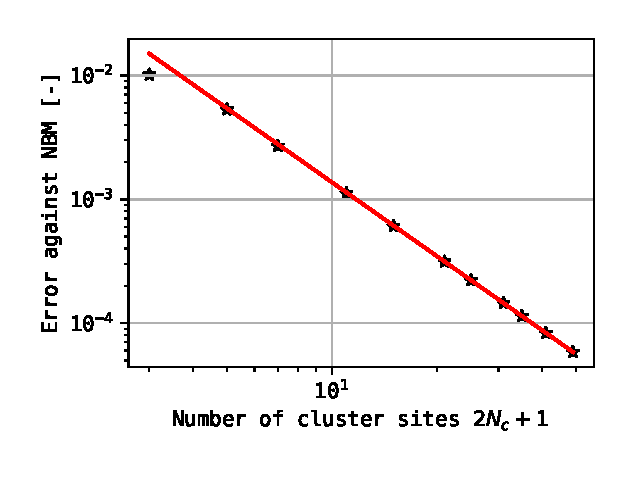
\includegraphics[width=0.8\textwidth]{figures/one_sys_err.eps}
	\caption{Error of CBG against BG for a homogeneous system with $N=500$. Compared for different cluster sizes in logarithmic scale. The slope of the linear approximation $-1.98$. }
	\label{fig:err_single_system}
\end{figure}

% subsection Error against BG (end)

Studying first results for the homogeneous sytem \ref{fig:err_single_system} with $N=500$, the data suggests that the error of CBG against the BG approaches an inversely quadratic relationship, meaning that the error scales with the cluster size to the power of $-2$. 

The divergence from this relationship at the start of plot could be credited to the fact that only one run for each cluster size has been recorded, thus could it be the statistical variance. More runs per cluster size would be needed to answer this question, and to make the claim that the inverse square relationship holds stronger. 

\subsection{Error against BG, inhomogeneous system} % (fold)
\label{sub:error_against_nbm_inhom}

Another interesting prospect to investigate is how the CBG behaves for inhomogeneous systems, as often more than not will the systems at hand be inhomogeneous. 

To investigate this will 5 different systems be defined; 1 homogeneous and 4 inhomogeneous. All systems will have a system size of $N=500$. Inhomogeneity will be introduced into the chemical potential by letting it be defined by a sine wave, and each system has different wave lengths in this wave. This can be seen as the correlation length of the inhomogenity of the system.  

A bias, amplitude and wavelength makes upp all these systems, where for the homogeneous has the bias $b = 1.0$, and the amplitude and wavelength are both set to 0. For the inhomogeneous systems will the bias be the same, while keeping the amplitude at $A = 2.0$ energy units, and the frequencies investigated are in the set $\{ 1.0, 3.0, 7.0, 11.0 \}$. 

The cluster sizes to be investigated will be in the span $N_c \in \{1, 2, 3, 4, 5, 6, 7, 8, 9, 10\}$, to cover as much granularity as possible. 

\begin{figure}[ht!]
	\centering
	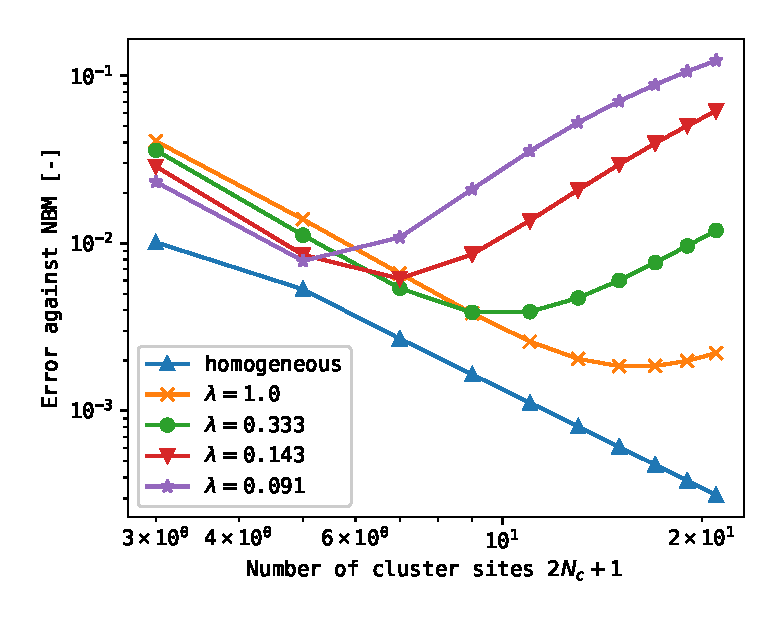
\includegraphics[width=0.8\textwidth]{figures/err_multiple_systems.eps}
	\caption{Error of CBG against BG compared for cluster sizes, in logarithmic scale. The cluster size is in units of the total system length and $\lambda$ denotes the wave/correlation length inherent to the wave like nature of the chemical potential in the inhomogeneous systems. }
	\label{fig:err_multiple_systems}
\end{figure}

The results of this is quite interesting \ref{fig:err_multiple_systems}. Comparing across the different systems, the homogeneous system has the overall best accuracy for all the cluster sizes. 

What is most interesting is the fact that the best accuracy for different systems is given at different cluster sizes. For instance, the lowest error for the system with $\lambda=1.0$ is given by the CBG with $N_c=7$, not the highest cluster size.

I plotted the correlation length / wave length of the system inhomogenity against the cluster size in the system and the data insinuates a linear relationship between these. Although, due to lack of data I could not draw any conclusions. The relationship between optimal cluster size and correlation lenght is something that would be worth investigating in the future. 

% subsection Error against BG (end)

\subsection{Time complexity of method}

Lastly we turn to the time complexity of the methods. For one iteration it is prettey simple \ref{fig:iteration_time}. Here we plot the time per solver iteration, and perform linear regression. Generally have the CBGs a slope of $1$, where as the BG has $2.4$. This means that the time per iteration for the CBG scales linearly with the system size, where as it scales according to $\sim N^{2.4}$ for the BG. This directly reflects the fact the each cluster is diagonalized for each site (linear) and diagonalization has a time complexity of $\mathcal{O} (n^{2.4})$. 

\begin{figure}[ht!]
	\centering
	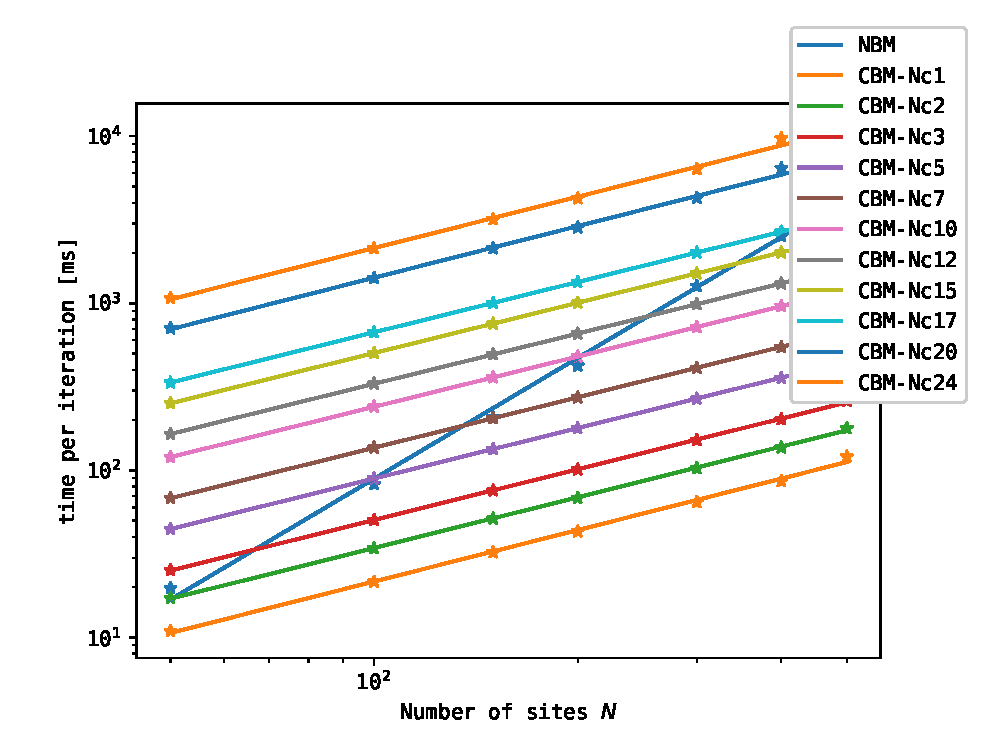
\includegraphics[width=0.8\textwidth]{figures/timing_analysis_time_per_iteration.eps}
	\caption{ Timing complexity of the BG and CBG for different cluster sizes for one iteration. For CBG is the slope of the fitted data overall $1.0$ and for BG $2.4$. }
	\label{fig:iteration_time}
\end{figure}

While only studying the time per iteration yields some insight, looking at the whole picture is arguably more important. In \ref{fig:solution_time} are the results of one simulation per number of sites per methods. (Note that we only have one simulation per point, not the most statistically sound. ) A similar trend can be seen here, though more stochastic. 

As expected will the CBG with $N_c = 1$ be the fastest to convergence, and the largest CBG method is the slowest. Looking at the slopes we can see that all CBGs have a similar scaling behavior, while the BG's time to convergence scales much worse. We can compare the slopes in tab. \ref{tab:slope_time-complexity}, where the most prominent observation is that the time to convergence for BG is scales about twice as much compared to all the CBGs. This reflects the inherent behavior of the method, where the diagonalization time scales with the total system size. The increase in slope for the CBGs with increasing method cluster size can be explained in a similar way, as the core is the diagonalization of the cluster matrices. 

\begin{figure}[ht!]
	\centering
	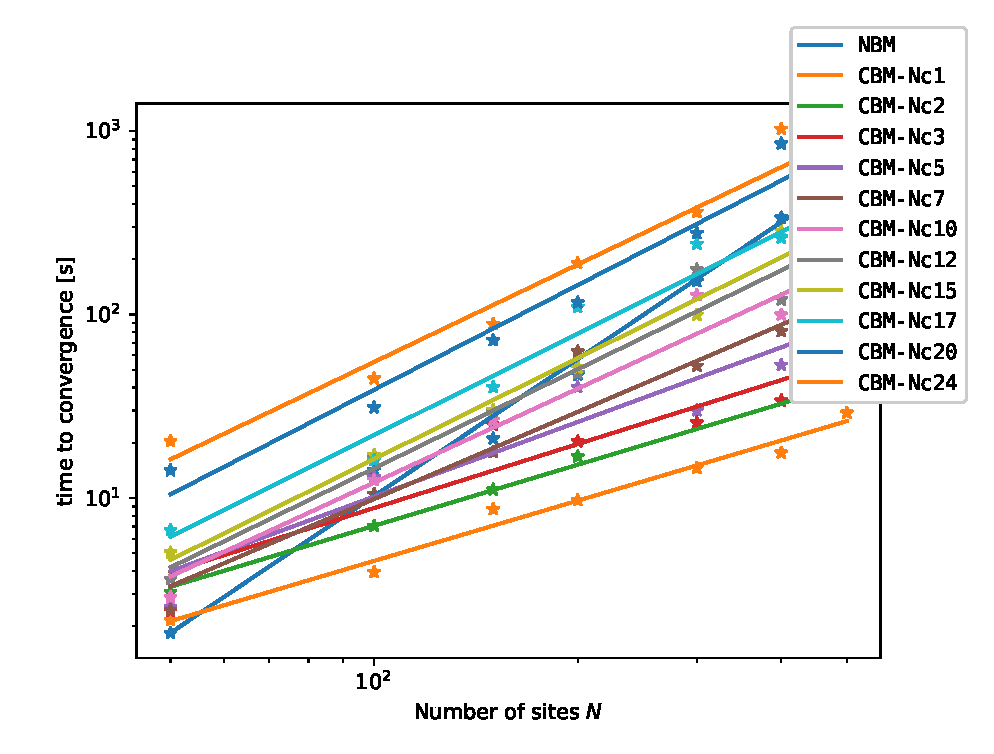
\includegraphics[width=0.8\textwidth]{figures/timing_analysis_tot_time.eps}
	\caption{ The time until convergence for the methods of different cluster sizes. }
	\label{fig:solution_time}
\end{figure}

More insight into the method can be yielded by studying the number of iterations it takes until convergence \ref{fig:num_iterations}. The largest slope is again for BG, whilst all other method has a lower slope value \ref{tab:slope_num_iteration}. More interesting is that the slope increases with the cluster size. The reason for this is most likely the way $\Delta$ is calculated from a cluster; through the mean. 

\begin{figure}[ht!]
	\centering
	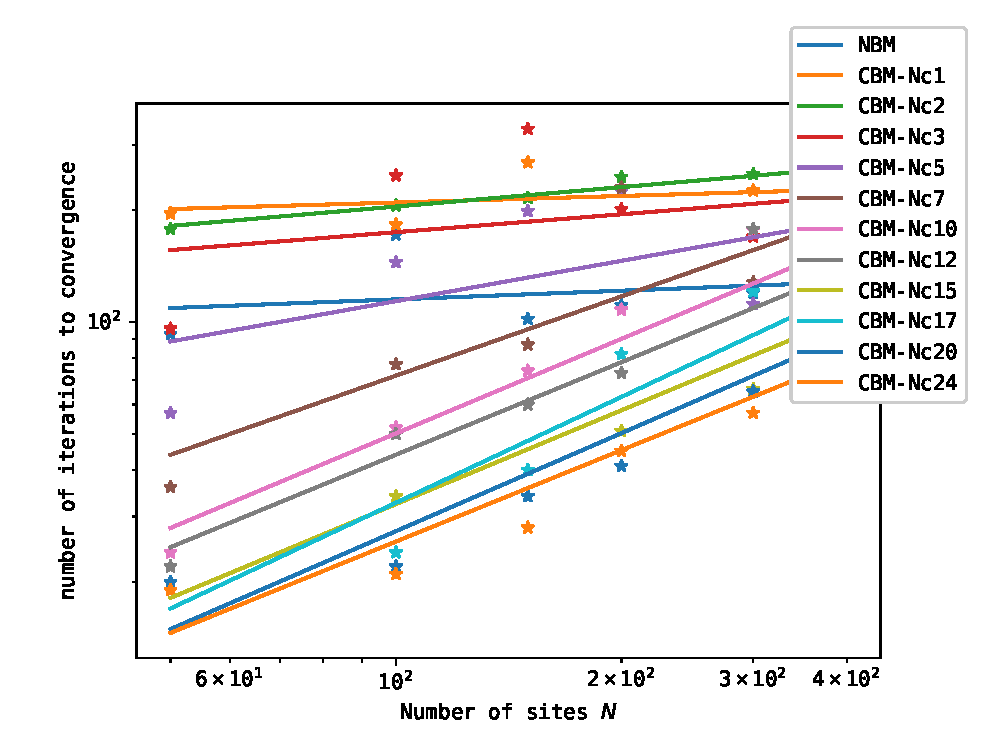
\includegraphics[width=0.8\textwidth]{figures/num_iterations.eps}
	\caption{ The number of iterations until convergence. The BG have a generally a constant number of iterations to convergence, while for CBG does the rate at which this number slightly increases increase with $N_c$.}
	\label{fig:num_iterations}
\end{figure}

\begin{table}
  \caption{Slope of time complexity for linear regression}\label{tab:slope_time-complexity}
  \begin{center}
    \begin{tabular}[c]{|c|c|}
      \hline
      Method & Slope \\
      \hline
      BG & $2.48$ \\ \hline \hline
      CBG, $N_c$ &  \\ \hline
      $1$ & 1.09 \\ \hline
      $2$ & 1.11 \\ \hline
      $3$ & 1.16 \\ \hline
      $5$ & 1.35 \\ \hline
      $7$ & 1.58 \\ \hline
      $10$ & 1.7 \\ \hline
      $12$ & 1.79 \\ \hline
      $15$ & 1.83 \\ \hline
      $17$ & 1.84 \\ \hline
      $20$ & 1.89 \\ \hline
      $24$ & 1.76 \\ \hline
      \hline
    \end{tabular}
  \end{center}
\end{table}

\begin{table}
  \caption{Slope of time complexity for linear regression}\label{tab:slope_num_iteration}
  \begin{center}
    \begin{tabular}[c]{|c|c|}
      \hline
      Method & Slope \\
      \hline
      BG & $0.08$ \\ \hline \hline
      CBG, $N_c$ &  \\ \hline
      $1$ & 0.07 \\ \hline
      $2$ & 0.1 \\ \hline
      $3$ & 0.15 \\ \hline
      $5$ & 0.35 \\ \hline
      $7$ & 0.57 \\ \hline
      $10$ & 0.7 \\ \hline
      $12$ & 0.79 \\ \hline
      $15$ & 0.83 \\ \hline
      $17$ & 0.84 \\ \hline
      $20$ & 0.87 \\ \hline
      $24$ & 0.74 \\ \hline
      \hline
    \end{tabular}
  \end{center}
\end{table}

\section{Discussion}\label{sec:discussion}

We have studied the cluster BdG method which was taken as a direct inspiration from the cluster Monte Carlo mathod \cite{kumarTravellingClusterApproximation2006} and compared it against the nominal BdG method to see if it is a competing method. Generally what can be seen is that the CBG has a lower accuracy compared to the BG, and the error of the CBG solutions for homogeneous systems is related inversely squared to the cluster size. 

What makes the CBG interesting to study is that the time complexity is slightly better than squared (a time complexity on around $~\mathcal{O}(n^{1.7})$), compared to the BG which has instead a time complexity of $~\mathcal{O}(n^{2.4})$. Furthermore, and perhaps the most interesting, is the sensitivity of the method to inhomogeneities in the underlying physical system. The data in this study suggests that CBGs with smaller cluster size works better for systems with lower correlation lengths in its inhomogeneities. An increase in the number of runs per data point would be needed to be more certain of the suggested claims.  

Due to the scope of this study was some things left out which are interesting for further studying. For instance, it would be very interesting to study different ways of obtaining the gap parameter from the cluster matrix using a weighted function instead of the mean, since it seems to affect the number of iterations needed for convergence. Secondly would validating the method against data from real systems an excellent way of investigating this method further. 

\section{Acknowledgements}

I would like to thank Mats Barkman for very insightful discussions which contributed a lot to this work. I also would like to thank the Theoretical Physics department at KTH for giving me access to their computation cluster in order to support this work. 

\onecolumn
% ref
\bibliographystyle{plain} % We choose the "plain" reference style
\bibliography{refs} % Entries are in the refs.bib file

\end{document}

pdflatex: --aux-directory=build
bibtex: build/% -use-directory=build

